\section{MPI One-Sided Communication}
\subsection{Required submission files}
\begin{enumerate}
  \item \hl{The updated \emph{gauss.c} file.}

  \item \hl{The new performance plots and description in the report.}

\end{enumerate}

\subsection{Questions}
\begin{enumerate}
  \item \hl{Which MPI-IO operations were applied to transform the code? Explain your choices.}
  There were several MPI-IO operations chosen to replace different parts of the code
  \begin{enumerate}
  \item 1) Reading in the matrix.
  
  We used an MPI_Read function to read the first two ints at the beginning of the matrix to determine matrix dimensions. We then used an MPI_File_set_view to separate the file into chunks and an MPI_File_read_all for all processes to read in the required matrix data. We chose to use MPI_File_set_view as the performance increase from a simple MPI_Read_at_all was significant.
  
  We used MPI_File_set_view and MPI_Read_all to read in the rhs data as well.
  
  \item 2) Writing the resulting solution vector
  We used an 
  
  \end{enumerate}
  
  \item \hl{What is "Data Sieving" and "2-Phase IO"? How do they help improve IO
performance?}

  \item \hl{Was the original implementation scalable in terms of IO performance?}
  The original implementation was not scalable in terms of IO performance. Only one process would read or write data. Thus, time would remain the same for IO regardless of the number of MPI processes.
  
  \item \hl{Was the original implementation scalable in terms of RAM storage?}
  The original implementation was not scalable in terms of RAM. When the program is run on a distributed memory system the entire matrix must fit inside the RAM associated with the processing unit executing the root process. This problem would not change regardless of the number of processing units (with their own memory) added.
  
  \item \hl{How much of the communication in the application was replaced or eliminated with MPI-IO? (Use
Vampir)}

  \item \hl{Were there any performance improvements due to the change to MPI-IO?}
  Yes, there was some performance improvements due to MPI-IO. We implemented the changes to MPI-IO on the baseline case to highlight the improvements.

\end{enumerate}
% % Figure example
% \begin{figure}[p] % h=here, t=top, b=bottom, p=(extra)page, !=force
%    \begin{center}
%      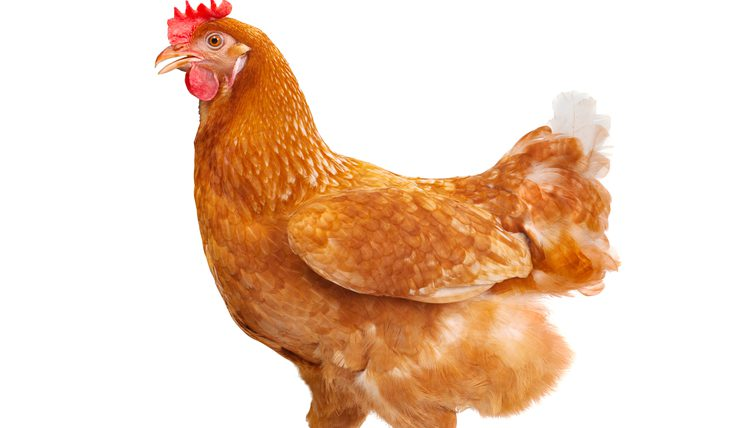
\includegraphics[width=.9\linewidth]{figure.png} % It searches in the Figures/ folder!
%      \caption{Caption text}
%      \label{fig:figureLabelName}
%    \end{center}
% \end{figure}
